% **************************************************
% Document Class Definition
% **************************************************
\documentclass[%
	paper=A4,					% paper size --> A4 is default in Germany
	twoside=true,				% onesite or twoside printing
	openright,					% doublepage cleaning ends up right side
	parskip=full,				% spacing value / method for paragraphs
	chapterprefix=true,			% prefix for chapter marks
	11pt,						% font size
	headings=normal,			% size of headings
	bibliography=totoc,			% include bib in toc
	listof=totoc,				% include listof entries in toc
	titlepage=on,				% own page for each title page
	captions=tableabove,		% display table captions above the float env
	draft=false,				% value for draft version
]{scrreprt}%

% **************************************************
% Debug LaTeX Information
% **************************************************
%\listfiles

% **************************************************
% Information and Commands for Reuse
% **************************************************
\newcommand{\ie}{\textit{i.e.,}\xspace}
\newcommand{\eg}{\textit{e.g.,}\xspace}
\newcommand{\etc}{\textit{etc.}\xspace}
\newcommand{\thesisTitle}{T\'{i}tulo de la tesis en ingl\'{e}s}
\newcommand{\thesisName}{Nombre de los autores de la tesis}
\newcommand{\thesisSubject}{Proyecto de grado}
\newcommand{\thesisDate}{Diciembre, 2019}
\newcommand{\thesisVersion}{1.0}

\newcommand{\thesisFirstReviewer}{Ph.D. Nicol\'{a}s Cardozo }
\newcommand{\thesisFirstReviewerUniversity}{\protect{Universidad de los Andes, Bogot\'{a}, Colombia}}
\newcommand{\thesisFirstReviewerDepartment}{Departamento de Ingenier\'{i}a de Sistemas y Computaci\'{o}n}

\newcommand{\thesisSecondReviewer}{Ph.D. Gabriele Bavota}
\newcommand{\thesisSecondReviewerUniversity}{\protect{Universit\`{a} della Svizzera italiana (USI), Lugano}}
\newcommand{\thesisSecondReviewerDepartment}{Faculty of Informatics }

\newcommand{\thesisFirstSupervisor}{Ph.D. Mario Linares V\'{a}squez}

\newcommand{\thesisUniversity}{\protect{Universidad de los Andes}}
\newcommand{\thesisUniversityDepartment}{Departamento de Ingenier\'{i}a de Sistemas y Computaci\'{o}n}
\newcommand{\thesisUniversityInstitute}{Facultad de Ingenier\'{i}a}
\newcommand{\thesisUniversityGroup}{The Software Design Lab}
\newcommand{\thesisUniversityCity}{Bogot\'{a}, Colombia}
\newcommand{\thesisUniversityStreetAddress}{Cra 1 \# 18A - 12}
\newcommand{\thesisUniversityPostalCode}{111711}



% **************************************************
% Load and Configure Packages
% **************************************************
\usepackage[T1]{fontenc}
\usepackage[utf8]{inputenc}		% defines file's character encoding
\usepackage[spanish]{babel} % babel system, adjust the language of the content
\usepackage[					% clean thesis style
	figuresep=colon,%
	sansserif=false,%
	hangfigurecaption=false,%
	hangsection=true,%
	hangsubsection=true,%
	colorize=full,%
	colortheme=bluemagenta,%
	bibsys=bibtex,%
	bibfile=bib-refs,%
	bibstyle=numeric,%
]{cleanthesis}
\usepackage[linesnumbered]{algorithm2e}
\usepackage{adjustbox}
\usepackage{listings,color}
\usepackage{amsfonts}
\usepackage{tcolorbox}
\usepackage{amssymb}
\usepackage{ifthen}
\lstset{
	language=xml,
	tabsize=2,
	%frame=lines,
	frame=shadowbox,
	rulesepcolor=\color{gray},
	xleftmargin=18pt,
	framexleftmargin=15pt,
	keywordstyle=\color{blue},
	commentstyle=\color{OliveGreen},
	stringstyle=\color[rgb]{0,0.43,0.72},
	numbers=left,
	numberstyle=\tiny,
	numbersep=4pt,
	breaklines=true,
	showstringspaces=false,
	basicstyle=\ttfamily\scriptsize,
	columns=fullflexible,
	emph={node,name,price},emphstyle={\color{magenta}}}

\colorlet{punct}{red!60!black}
\definecolor{background}{HTML}{EEEEEE}
\definecolor{delim}{RGB}{20,105,176}
\colorlet{numb}{magenta!60!black}
\lstdefinelanguage{json}{
	basicstyle=\ttfamily\scriptsize,
	numbers=left,
	numberstyle=\scriptsize,
	stepnumber=1,
	numbersep=8pt,
	showstringspaces=false,
	breaklines=true,
	frame=shadowbox,
	literate=
	*{0}{{{\color{numb}0}}}{1}
	{1}{{{\color{numb}1}}}{1}
	{2}{{{\color{numb}2}}}{1}
	{3}{{{\color{numb}3}}}{1}
	{4}{{{\color{numb}4}}}{1}
	{5}{{{\color{numb}5}}}{1}
	{6}{{{\color{numb}6}}}{1}
	{7}{{{\color{numb}7}}}{1}
	{8}{{{\color{numb}8}}}{1}
	{9}{{{\color{numb}9}}}{1}
	{:}{{{\color{punct}{:}}}}{1}
	{,}{{{\color{punct}{,}}}}{1}
	{\{}{{{\color{delim}{\{}}}}{1}
	{\}}{{{\color{delim}{\}}}}}{1}
	{[}{{{\color{delim}{[}}}}{1}
	{]}{{{\color{delim}{]}}}}{1},
}

\lstloadlanguages{xml}
\renewcommand{\lstlistingname}{Code example}% Listing -> Algorithm
\renewcommand{\lstlistlistingname}{List of \lstlistingname s}


\hypersetup{					% setup the hyperref-package options
	pdftitle={\thesisTitle},	% 	- title (PDF meta)
	pdfsubject={\thesisSubject},% 	- subject (PDF meta)
	pdfauthor={\thesisName},	% 	- author (PDF meta)
	plainpages=false,			% 	-
	colorlinks=false,			% 	- colorize links?
	pdfborder={0 0 0},			% 	-
	breaklinks=true,			% 	- allow line break inside links
	bookmarksnumbered=true,		%
	bookmarksopen=true			%
}

\newcommand{\nb}[2]{
	\fbox{\bfseries\sffamily\scriptsize#1}
	{\small$\blacktriangleright$\textit{#2}$\blacktriangleleft$}}
\newcommand\MARIO[1]{\textcolor{red}{\nb{MARIO}{#1}}}
\newcommand\SANTIAGO[1]{\textcolor{orange}{\nb{SANTIAGO}{#1}}}
% **************************************************
% Document CONTENT
% **************************************************
\begin{document}

% --------------------------
% rename document parts
% --------------------------
%\renewcaptionname{ngerman}{\figurename}{Abb.}
%\renewcaptionname{ngerman}{\tablename}{Tab.}
\renewcaptionname{spanish}{\figurename}{Fig.}
\renewcaptionname{spanish}{\tablename}{Tab.}

% --------------------------
% Front matter
% --------------------------
\pagenumbering{roman}			% roman page numbing (invisible for empty page style)
\pagestyle{empty}				% no header or footers
% !TEX root = ../thesis-example.tex
%
% ------------------------------------  --> cover title page
\begin{titlepage}
	\pdfbookmark[0]{Cover}{Cover}
	\flushright
	\hfill
	\vfill
	{\LARGE\thesisTitle \par}
	\rule[5pt]{\textwidth}{.4pt} \par
	{\Large\thesisName}
	\vfill
	\textit{\large\thesisDate} \\
	Version: \thesisVersion
\end{titlepage}


% ------------------------------------  --> main title page
\begin{titlepage}
	\pdfbookmark[0]{Titlepage}{Titlepage}
	\tgherosfont
	\centering

	Bogotá, Colombia \\[4mm]
	
\includegraphics[width=6cm]{img/logo-uniandes.png} \\[2mm]
	\textsf{\thesisUniversityDepartment} \\
	\textsf{\thesisUniversityInstitute} \\
	\textsf{\thesisUniversityGroup} \\

	\vfill
	{\large \thesisSubject} \\[5mm]
	{\LARGE \color{ctcolortitle}\textbf{\thesisTitle} \\[10mm]}
	{\Large \thesisName} \\

	\vfill
		\begin{minipage}[t]{.27\textwidth}
		\raggedleft
		\textit{Asesor}
	\end{minipage}
	\hspace*{15pt}
	\begin{minipage}[t]{.65\textwidth}
		{\Large \thesisFirstSupervisor} \\
		{\small \thesisFirstReviewerDepartment} \\[-1mm]
		{\small \thesisFirstReviewerUniversity}
	\end{minipage} \\[5mm]

	\thesisDate \\

\end{titlepage}


% ------------------------------------  --> lower title back for single page layout
\hfill
\vfill
{
	\small
	\textbf{\thesisName} \\
	\textit{\thesisTitle} \\
	\thesisSubject, \thesisDate \\
	Asesor: \thesisFirstSupervisor\\[1.5em]
	\textbf{\thesisUniversity} \\
	\textit{\thesisUniversityGroup} \\
	\thesisUniversityInstitute \\
	\thesisUniversityDepartment \\
	\thesisUniversityStreetAddress \\
	\thesisUniversityPostalCode\ and \thesisUniversityCity
}
		% INCLUDE: all titlepages
\cleardoublepage

\pagestyle{plain}				% display just page numbers
% !TEX root = ../thesis-example.tex
%
\pdfbookmark[0]{Resumen}{Resumen}
\chapter*{Resumen}
\label{sec:abstract}
\vspace*{-10mm}
La complejidad y el rápido crecimiento del mercado de aplicaciones móviles, hace necesario que los desarrolladores deban automatizar tareas de pruebas y control de calidad sobre los productos de software. El presente documento presenta un enfoque de generación automática de pruebas, basado en el análisis de multi-modelos: estructuras con información sobre una aplicación móvil y su contexto que permiten definir casos de uso de las aplicaciones sin intervención humana. De forma automática se crean pruebas basadas en \textit{Espresso}, una herramienta enfocada en los desarrolladores, que les permite integrar sus pruebas: los ladrillos que permiten construir entornos con integración continua.

\vspace*{20mm}
		% INCLUDE: the abstracts (english and german)
\cleardoublepage
%
%% !TEX root = ../thesis-example.tex
%
\pdfbookmark[0]{Acknowledgement}{Acknowledgement}
\chapter*{Acknowledgement}
\label{sec:acknowledgement}
\vspace*{-10mm}

\Blindtext[2][2]
 % INCLUDE: acknowledgement
%\cleardoublepage
%
\setcounter{tocdepth}{2}		% define depth of toc
\tableofcontents				% display table of contents
\cleardoublepage

% --------------------------
% Body matter
% --------------------------
\pagenumbering{arabic}			% arabic page numbering
\setcounter{page}{1}			% set page counter
\pagestyle{maincontentstyle} 	% fancy header and footer

% !TEX root = ../thesis-example.tex
%
\chapter{Introducción}
\label{sec:intro}

\section{Motivación}

Las aplicaciones móviles se han convertido en una gran parte de nuestras vidas. De acuerdo a Statista \cite{MobileStatista}, el número de aplicaciones disponibles en Google Play Store para el primer cuarto de 2018 fue de 3.8 millones. En 2017 fueron descargadas 178.1 billones de aplicaciones en el mundo. A medida que crece este mercado, también lo hace la necesidad de mejorar cada etapa del proceso de desarrollo para entregar un producto de calidad de manera eficiente. Una de estas es la etapa de pruebas. Mediante esta los desarrolladores pueden asegurar la calidad del software y por consiguiente la satisfacción del cliente.

En el desarrollo de aplicaciones móviles, es especialmente crítico asegurar que el producto está libre de errores. Hay una gran variedad de alternativas presentadas a los usuarios, y esta facilidad de adquisición hace para ellos más fácil tomar la decisión de cambiar entre ellas. Es por esto que un error en la aplicación puede traducirse en una gran pérdida de clientes.

Las pruebas en aplicaciones móviles se enfrentan a una variedad de retos, uno de estos es la des-fragmentación de plataformas móviles. Esto se refiere al hecho de que hay un gran número de combinaciones de dispositivos con sus sistemas operativos. Por lo tanto, la tarea de realizar pruebas en una aplicación móvil se hace aún más complicada. No solo tiene el tester que asegurar el correcto funcionamiento de la aplicación en un SO (Android, iOS), sino que también se deben tener en cuenta las diferentes modificaciones que son realizadas por cada OEM (Manufacturador original del equipo). Dado que este problema tiene mayor impacto para el caso de Android, el proyecto se basará en dicho sistema operativo.
Por otro lado, las aplicaciones móviles, en comparación con las de escritorio, están sujetas a muchas más variables que pueden influenciar su correcto funcionamiento. Los recursos disponibles en un dispositivo móvil son mucho más limitados que los que se encuentran en un computador. Además, se deben tener en cuenta sensores, batería, otras aplicaciones corriendo en el dispositivo, etc.

Por consiguiente, al tener una gran variedad de retos en este campo, proponemos abordar el problema mediante el uso de multi-modelos para generar estas pruebas. Basados en la extracción de modelos propuesta en Automated Extraction of Augmented Models for Android Apps (RIP tool) \cite{LinanAutomatedApps} y CEL \cite{Linares-Vasquez2017ContinuousTesting}, proponemos una herramienta para generar tests de manera automática que tiene en cuenta los tres modelos (contexto, dominio y GUI). Al tener en consideración la información proporcionada por estos modelos, se generarán tests más fieles a la realidad, asegurando mayor cobertura en casos de prueba.

\section{Objetivos}

\begin{itemize}
	\item Generar casos de prueba de 'esquina' basados en las probables causas de error encontradas con los modelos.
	\item Generar casos de pruebas basados en los cambios contextuales de la aplicación (conectividad, batería, etc).
	\item Proveer al usuario con una visualización de la ejecución de las pruebas a través de una aplicación web.
\end{itemize}

\section{Resultados esperados}
Al finalizar el proyecto, será posible para el tester generar varios casos de prueba de manera automatizada, considerando los posibles factores que pueden influenciar la aplicación móvil. Esto reducirá el costo de tener que probar la aplicación de manera manual o programando los casos de prueba.
\section{Resultados alcanzados}
Se construyó una herramienta que permite al desarrollador generar casos de prueba que se pueden reproducir con el framework Espresso. Estos casos tienen en cuenta el modelo GUI extraído por RIP junto con el modelo de dominio y los cambios contextuales producidos en la aplicación. Se decidió usar Espresso debido a que es la herramienta oficial propuesta por Google, además de estar ampliamente documentado para su fácil modificación por parte del desarrollador/usuario.
 % INCLUDE: introduction
% !TEX root = ../thesis-example.tex
%
\chapter{Trabajo relacionado y herramientas existentes}
\label{chapter2}

\section{Generación automática de pruebas}
Para la generación de pruebas existen diversas herramientas que abarcan el problema de distintas maneras. A continuación se presenta un análisis de las herramientas que se acercan más a nuestra propuesta, sin embargo difieren en que solo se basan en el modelo de GUI.

\subsection{Barista}
Barista \cite{Fazzini2017} es una herramienta \textit{record and replay} en la cual el tester realiza una prueba de manera manual sobre la GUI de la aplicación. Después, un caso de prueba es codificado para poder ser reproducido en otros dispositivos múltiples veces. A pesar de que este enfoque provee una manera fácil de generar un caso de prueba, el tester se ve obligado a realizar manualmente cada prueba al menos una vez interactuando con la GUI.

\subsection{MobiGUITAR}
A diferencia de Barista, MobiGUITAR \cite{MobiGUITAR} realiza la interacción y extracción de eventos de la aplicación de manera automática usando GUI Ripping. Mediante esta técnica, se genera una modelo de máquina de estado que representa todos los eventos de la aplicación. A pesar de automatizar el paso de creación de la prueba, esta herramienta no tiene en cuenta los cambios contextuales del dispositivo.

\subsection{Firebase Test Lab}
Este servicio \cite{firebase} en la nube ofrecido por Google, permite al usuario subir el apk de la aplicación y correr varios tipos de pruebas en la aplicación. Sin embargo, similar a las herramientas anteriores, se basa en exploración de GUI. Además, posee un costo adicional si se desea probar en un mayor número de dispositivos.

\subsection{Sapienz}
Sapienz\cite{sapienz} utiliza un enfoque multi-objetivo para la exploración y generación de casos de prueba. Esto hace que se obtengan tests mas cortos que maximizan	 su cobertura. Una ventaja de esta herramienta es que se pueden generar pruebas solo con el apk de la aplicación. Sin embargo no se tienen en cuenta los cambios contextuales de la aplicación.
 % INCLUDE: related work
\chapter{RIP Tests Generator}
\label{chapter3}

\section{Solución propuesta}
Como fue mencionado anteriormente, uno de los principales problemas a la hora de generar casos de prueba, es poder tener en cuenta los diferentes cambios de contexto y los tipos de entidades encontrados en la aplicación. Por esto, la generación de tests de esta herramienta está basada en los diferentes modelos encontrados con la herramienta  \textbf{RIP}\cite{LinanAutomatedApps}. Concretamente se tienen definidos tres modelos: GUI, contexto y dominio, los cuales se basan en lo propuesto en CEL\cite{Linares-Vasquez2017ContinuousTesting}.

El modelo GUI es extraído mediante la técnica GUI ripping, en donde se realiza una exploración de la interfaz de la aplicación, generando un diagrama de estados que representan las actividades y eventos de transición entre ellas. Para el modelo de dominio, se realiza un análisis de los componentes encontrados en los XML's de la aplicación, para así describir los datos que pueden ser introducidos o producidos. Finalmente, mediante el diagrama de contexto se conocen las condiciones externas que podrían afectar el correcto funcionamiento de la aplicación. Información como sensores,  uso de batería, o conectividad es recolectada en este modelo.

Una vez se tiene la información sobre los diversos modelos, se propone crear \textbf{RIP Tests Generator}, una herramienta que genere de manera automática los archivos de prueba usando Espresso. Este es el framework sugerido por Google con el fin de escribir pruebas de para aplicaciones Android.



\section{Arquitectura de la solución}

\textbf{RIP Tests Generator} genera tests después de que \textbf{RIP} termina la ejecución, lo que permite el desacoplamiento de las dos herramientas. En este caso, \textbf{RIP} \cite{LinanAutomatedApps} puede mejorar o cambiar sus algoritmos de exploración dinámica sobre aplicaciones móviles, manteniendo la compatibilidad con \textbf{RIP Tests Generator}. La figura \ref{procesoTests} presenta el resumen del proceso de generación de tests a partir de los archivos obtenidos mediante la ejecución de RIP.

\begin{figure}[h]
	\centering
	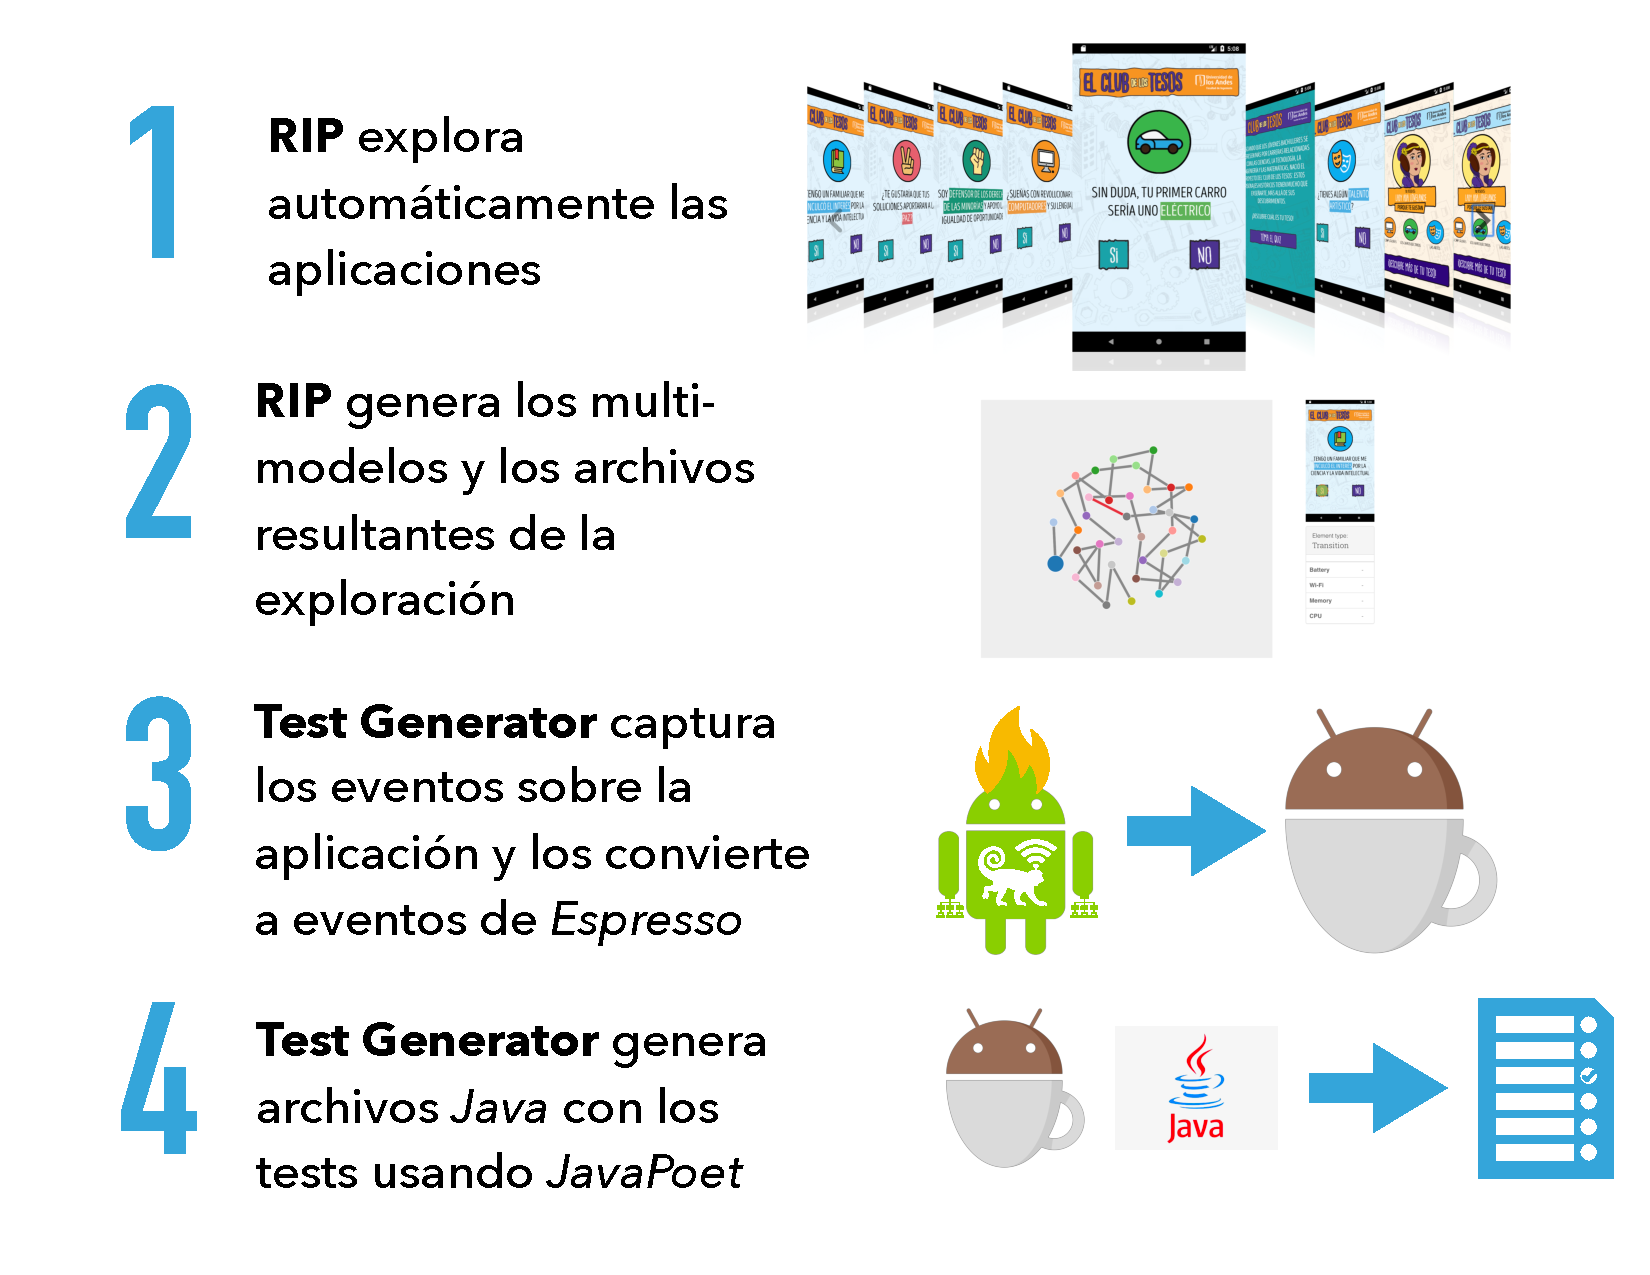
\includegraphics[width=1\textwidth]{img/procesoTests.pdf}
	\vspace{-0.5cm}
	\caption{Proceso de generación automática de tests}
	\label{procesoTests}
\end{figure} 

Test Generator es un componente acoplado con RIP que es ejecutado cuando se termina la exploración de la aplicación. Para esto, se creó la clase TestCaseBuilder.java que toma los datos proporcionados en el archivo tree.json y traduce los eventos a comandos de espresso.


Para la generación de pruebas se definieron los siguientes eventos, basados en los generados por RIP:

\textbf{TAP} : Cuando se tiene esta acción se traduce a un evento de hacer click en el botón o campo con el id proporcionado. Para implementar esta acción en espresso, se utiliza el comando \textit{onView(withId(id)).perform(click())}.

\textbf{INPUT} :  Al detectar un evento de campo de texto, con ayuda del modelo de dominio se detecta el tipo de dato a ingresar. Para esto se tiene la posibilidad de crear texto de manera aleatoria en un rango de caracteres normal o con una gran cantidad de estos con el fin de probar los limites de estos campos. Esta acción es implementada mediante el comando \textit{onView(withId(id)).perform(replaceText("randomtext"),closeSoftKeyboard());}



\section{Requisitos técnicos para la generación automática de pruebas}
Con el fin de que el desarrollador no tenga ningún inconveniente usando la herramienta, se definieron los siguientes requisitos técnicos:
\begin{enumerate}
	\item Al estar integrada con \textbf{RIP}\cite{LinanAutomatedApps}, se debe tener instalado ADB y correr el software en dispositivos rooteados o emuladores.
	\item El desarrollador debe tener acceso al código fuente de la aplicación, ya que los archivos de prueba generados solo pueden ser ejecutados si son empaquetados junto al código fuente.
	\item Es necesario htreeacer los cambios pertinentes en el build.gradle del proyecto para importar las dependencias utilizadas en los casos de prueba. Un ejemplo de esto es encontrado en la figura \ref{dependencies}.
	

\end{enumerate} 

	\begin{figure}[h]
	\centering
	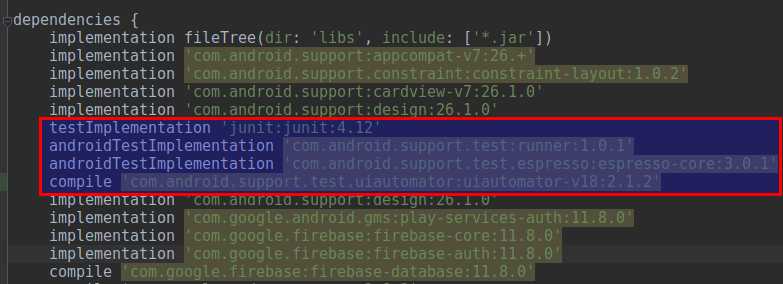
\includegraphics[width=1\textwidth]{img/dependencies.png}
	\vspace{-0.5cm}
	\caption{Ejemplo de archivo build.gradle con las dependencias necesarias para la ejecución de las pruebas}
	\label{dependencies}
\end{figure} 


\section{Generación automática de una prueba}
Para generar una prueba se hace uso del archivo tree.json \textbf{RIP}, el cual contiene un grafo donde las actividades corresponden a los nodos y los links a los eventos que disparan una transición entre dos estados. Cada nodo contiene la información del modelo de dominio con el tipo de datos que se encuentran. Además, se tienen los diferentes indicadores de contexto en cada estado, donde se pueden ver datos como batería, conectividad de internet, etc.

Dicho archivo es el que se utiliza como insumo para generar los casos de prueba mediante RIP Tests Generator. Gracias a la librería JavaPoet \cite{JavaPoet} se genera un archivo .java que contiene el código fuente de la prueba. Para esto, se tiene en cuenta la información obtenida del grafo generado por RIP y se hace una traducción de cada acción a ser ejecutada en la prueba.

Mediante el modelo GUI se pueden generar los eventos de transición. Por ejemplo, si la acción que produjo un cambio de estado es un tap en el botón con id 'buttonJugar', entonces esto será traducido como un \textit{onView(withId(R.id.buttonJugar)).perform(click());}. Para generar esto, se tiene un método auxiliar que retorna la línea de código correspondiente. Al analizar el grafo, según el tipo de acción encontrada se genera una línea de código diferente. Este proceso se puede evidenciar en el ejemplo de la figura \ref{gentest}.

Respecto a la implementación de la generación de código con JavaPoet se debe mencionar que las librerías correctamente declaradas son importadas de manera automática en el archivo generado. Además, el paquete donde debe ser ubicado el archivo fuente se inserta de manera correcta. Finalmente, después de cada acción, se toma una captura de pantalla que será posteriormente extraída del dispositivo para generar el reporte de visualización web.

El algoritmo propuesto para la generación de la prueba es el siguiente:

\begin{enumerate}
	\item Tomar la secuencia de eventos generada por RIP y guardarlos en una lista.
	\item Realizar la acción de tomar una captura de pantalla antes de cada transición.
	\item Según cada evento generar la línea de código correspondiente en el lenguaje espresso.
	\item Si se tiene un cambio de contexto en el nodo, realizar la traducción correspondiente.
	\item Con la ayuda de JavaPoet, generar los campos usados por Espresso. Como lo son la ActivityTestRule, para indicar en que actividad iniciar la aplicación, y los permisos de escritura y lectura para las capturas de pantalla.
	\item Finalmente, para la correcta ejecución de la prueba, se genera un archivo ejecutable que se encarga de empaquetar el apk, correr las pruebas encontradas en el paquete test, y extraer las capturas de pantalla del dispositivo.
\end{enumerate}
Un ejemplo de la prueba obtenida como resultado puede ser evidenciado en la figura \ref{pruebaresultado}

\begin{figure}[h]
	\centering
	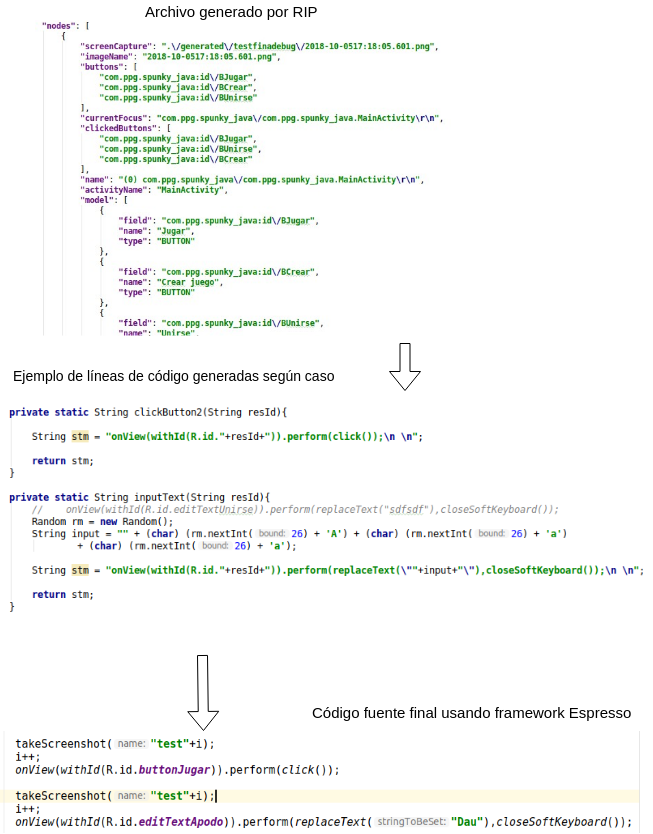
\includegraphics[width=1\textwidth]{img/GeneracionPrueba.png}
	\vspace{-0.5cm}
	\caption{Proceso de traducción y generación de prueba}
	\label{gentest}
\end{figure} 

\begin{figure}[h]
	\centering
	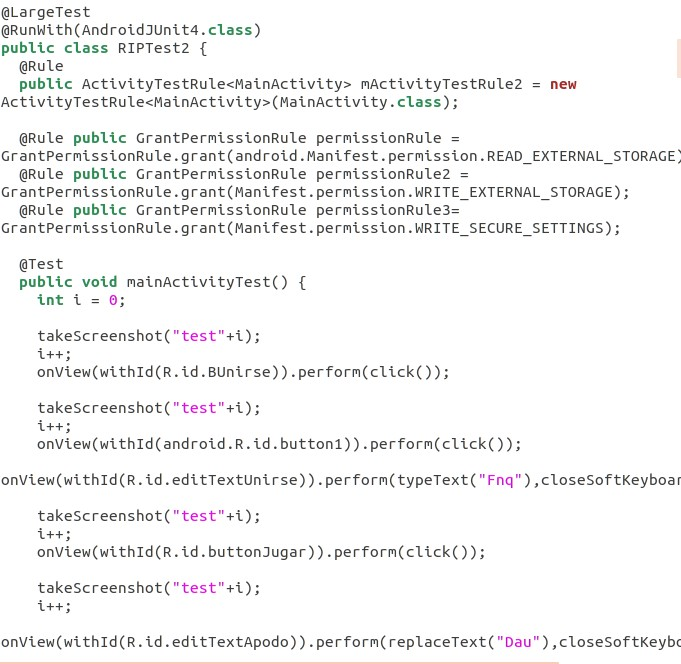
\includegraphics[width=1\textwidth]{img/pruebaResultado.jpg}
	\vspace{-0.5cm}
	\caption{Prueba generada}
	\label{pruebaresultado}
\end{figure} 







	
	% INCLUDE: system
% !TEX root = ../thesis-example.tex
%
\chapter{Conclusiones}
\label{chapter5}

Durante el desarrollo del proyecto se lograron la mayoría de los objetivos propuestos, y se construyó un generador automático de pruebas funcional. A continuación se presentan las conclusiones del proceso y el trabajo futuro.

\section{Objetivos cumplidos}

Gracias a la implementación de esta herramienta se obtuvo un producto inicial que genera pruebas basado en los modelos producidos por RIP. Durante el proceso se adquirieron conocimientos sobre exploración de aplicaciones móviles y generación de código java. Además, se logró el objetivo principal, integrar multi-modelos en la generación de pruebas. Se tuvieron en cuenta los 3 modelos, contexto, dominio y GUI, lo cual es el factor que diferencia la solución de otras ya existentes.


\section{Limitaciones del desarrollo}
\begin{itemize}
	\item Como se mencionó anteriormente, la generación de pruebas está enfocada exclusivamente en aplicaciones Android. Esto porque es el sistema operativo donde se presentan mayores problemas de desfragmentación y ofrece la facilidad de explorar las aplicaciones mediante herramientas como ADB.
	
	\item Debido al alcance del proyecto, el desarrollador debe tener el código fuente de la aplicación para poder ejecutar la prueba
	
	\item La extracción del modelo de dominio está basada en los componentes básicos de Android, por lo tanto, los que sean personalizados o de otras librerías no serán reconocidos en dicho modelo.
	
	\item El desarrollador debe tener derechos de superusuario sobre el dispositivo o correr las pruebas en un emulador para realizar algunas acciones.
	
	
\end{itemize}


\section{Trabajo futuro}

El proyecto presenta varias oportunidades de mejora como lo son:

\begin{itemize}
	\item Ejecución de la prueba sin tener acceso al código fuente.
	\item Extender los componentes que son detectados en los diferentes modelos.
	\item Tener una interfaz para el uso de la herramienta.
	\item Permitir al usuario ingresar valores personalizados para campos que lo requieran como los de usuario y contraseña.
	
	
\end{itemize}

 % INCLUDE: conclusion
\cleardoublepage

\printbibliography


\cleardoublepage

\listoffigures
\clearpage

%\listoftables
%\clearpage

% !TEX root = ../thesis-example.tex
%
\pagestyle{empty}
\hfill
\vfill
\pdfbookmark[0]{Colophon}{Colophon}
\section*{Colophon}

Este documento fue escrito en \LaTeXe. Usa el estilo \textit{Clean Thesis} desarrollado por Ricardo Langner.
%\cleardoublepage
%% !TEX root = ../thesis-example.tex
%
%************************************************
% Declaration
%************************************************
\pdfbookmark[0]{Declaration}{Declaration}
\chapter*{Declaration}
\label{sec:declaration}
\thispagestyle{empty}

You can put your declaration here, to declare that you have completed your work solely and only with the help of the references you mentioned.

\bigskip

\noindent\textit{\thesisUniversityCity, \thesisDate}

\smallskip

\begin{flushright}
	\begin{minipage}{5cm}
		\rule{\textwidth}{1pt}
		\centering\thesisName
	\end{minipage}
\end{flushright}

%*****************************************
%*****************************************

\clearpage
\newpage
\mbox{}

% **************************************************
% End of Document CONTENT
% **************************************************
\end{document}
